% Options for packages loaded elsewhere
\PassOptionsToPackage{unicode}{hyperref}
\PassOptionsToPackage{hyphens}{url}
%
\documentclass[
]{article}
\usepackage{amsmath,amssymb}
\usepackage{iftex}
\ifPDFTeX
  \usepackage[T1]{fontenc}
  \usepackage[utf8]{inputenc}
  \usepackage{textcomp} % provide euro and other symbols
\else % if luatex or xetex
  \usepackage{unicode-math} % this also loads fontspec
  \defaultfontfeatures{Scale=MatchLowercase}
  \defaultfontfeatures[\rmfamily]{Ligatures=TeX,Scale=1}
\fi
\usepackage{lmodern}
\ifPDFTeX\else
  % xetex/luatex font selection
\fi
% Use upquote if available, for straight quotes in verbatim environments
\IfFileExists{upquote.sty}{\usepackage{upquote}}{}
\IfFileExists{microtype.sty}{% use microtype if available
  \usepackage[]{microtype}
  \UseMicrotypeSet[protrusion]{basicmath} % disable protrusion for tt fonts
}{}
\makeatletter
\@ifundefined{KOMAClassName}{% if non-KOMA class
  \IfFileExists{parskip.sty}{%
    \usepackage{parskip}
  }{% else
    \setlength{\parindent}{0pt}
    \setlength{\parskip}{6pt plus 2pt minus 1pt}}
}{% if KOMA class
  \KOMAoptions{parskip=half}}
\makeatother
\usepackage{xcolor}
\usepackage[margin=1in]{geometry}
\usepackage{color}
\usepackage{fancyvrb}
\newcommand{\VerbBar}{|}
\newcommand{\VERB}{\Verb[commandchars=\\\{\}]}
\DefineVerbatimEnvironment{Highlighting}{Verbatim}{commandchars=\\\{\}}
% Add ',fontsize=\small' for more characters per line
\usepackage{framed}
\definecolor{shadecolor}{RGB}{248,248,248}
\newenvironment{Shaded}{\begin{snugshade}}{\end{snugshade}}
\newcommand{\AlertTok}[1]{\textcolor[rgb]{0.94,0.16,0.16}{#1}}
\newcommand{\AnnotationTok}[1]{\textcolor[rgb]{0.56,0.35,0.01}{\textbf{\textit{#1}}}}
\newcommand{\AttributeTok}[1]{\textcolor[rgb]{0.13,0.29,0.53}{#1}}
\newcommand{\BaseNTok}[1]{\textcolor[rgb]{0.00,0.00,0.81}{#1}}
\newcommand{\BuiltInTok}[1]{#1}
\newcommand{\CharTok}[1]{\textcolor[rgb]{0.31,0.60,0.02}{#1}}
\newcommand{\CommentTok}[1]{\textcolor[rgb]{0.56,0.35,0.01}{\textit{#1}}}
\newcommand{\CommentVarTok}[1]{\textcolor[rgb]{0.56,0.35,0.01}{\textbf{\textit{#1}}}}
\newcommand{\ConstantTok}[1]{\textcolor[rgb]{0.56,0.35,0.01}{#1}}
\newcommand{\ControlFlowTok}[1]{\textcolor[rgb]{0.13,0.29,0.53}{\textbf{#1}}}
\newcommand{\DataTypeTok}[1]{\textcolor[rgb]{0.13,0.29,0.53}{#1}}
\newcommand{\DecValTok}[1]{\textcolor[rgb]{0.00,0.00,0.81}{#1}}
\newcommand{\DocumentationTok}[1]{\textcolor[rgb]{0.56,0.35,0.01}{\textbf{\textit{#1}}}}
\newcommand{\ErrorTok}[1]{\textcolor[rgb]{0.64,0.00,0.00}{\textbf{#1}}}
\newcommand{\ExtensionTok}[1]{#1}
\newcommand{\FloatTok}[1]{\textcolor[rgb]{0.00,0.00,0.81}{#1}}
\newcommand{\FunctionTok}[1]{\textcolor[rgb]{0.13,0.29,0.53}{\textbf{#1}}}
\newcommand{\ImportTok}[1]{#1}
\newcommand{\InformationTok}[1]{\textcolor[rgb]{0.56,0.35,0.01}{\textbf{\textit{#1}}}}
\newcommand{\KeywordTok}[1]{\textcolor[rgb]{0.13,0.29,0.53}{\textbf{#1}}}
\newcommand{\NormalTok}[1]{#1}
\newcommand{\OperatorTok}[1]{\textcolor[rgb]{0.81,0.36,0.00}{\textbf{#1}}}
\newcommand{\OtherTok}[1]{\textcolor[rgb]{0.56,0.35,0.01}{#1}}
\newcommand{\PreprocessorTok}[1]{\textcolor[rgb]{0.56,0.35,0.01}{\textit{#1}}}
\newcommand{\RegionMarkerTok}[1]{#1}
\newcommand{\SpecialCharTok}[1]{\textcolor[rgb]{0.81,0.36,0.00}{\textbf{#1}}}
\newcommand{\SpecialStringTok}[1]{\textcolor[rgb]{0.31,0.60,0.02}{#1}}
\newcommand{\StringTok}[1]{\textcolor[rgb]{0.31,0.60,0.02}{#1}}
\newcommand{\VariableTok}[1]{\textcolor[rgb]{0.00,0.00,0.00}{#1}}
\newcommand{\VerbatimStringTok}[1]{\textcolor[rgb]{0.31,0.60,0.02}{#1}}
\newcommand{\WarningTok}[1]{\textcolor[rgb]{0.56,0.35,0.01}{\textbf{\textit{#1}}}}
\usepackage{graphicx}
\makeatletter
\def\maxwidth{\ifdim\Gin@nat@width>\linewidth\linewidth\else\Gin@nat@width\fi}
\def\maxheight{\ifdim\Gin@nat@height>\textheight\textheight\else\Gin@nat@height\fi}
\makeatother
% Scale images if necessary, so that they will not overflow the page
% margins by default, and it is still possible to overwrite the defaults
% using explicit options in \includegraphics[width, height, ...]{}
\setkeys{Gin}{width=\maxwidth,height=\maxheight,keepaspectratio}
% Set default figure placement to htbp
\makeatletter
\def\fps@figure{htbp}
\makeatother
\setlength{\emergencystretch}{3em} % prevent overfull lines
\providecommand{\tightlist}{%
  \setlength{\itemsep}{0pt}\setlength{\parskip}{0pt}}
\setcounter{secnumdepth}{-\maxdimen} % remove section numbering
\ifLuaTeX
  \usepackage{selnolig}  % disable illegal ligatures
\fi
\usepackage{bookmark}
\IfFileExists{xurl.sty}{\usepackage{xurl}}{} % add URL line breaks if available
\urlstyle{same}
\hypersetup{
  pdftitle={Analise exploratoria},
  pdfauthor={João Lucas},
  hidelinks,
  pdfcreator={LaTeX via pandoc}}

\title{Analise exploratoria}
\author{João Lucas}
\date{2024-08-05}

\begin{document}
\maketitle

\section{Análise exploratório de
dados}\label{anuxe1lise-exploratuxf3rio-de-dados}

\texttt{\{r\}\ \{r\ setup,\ include=FALSE\}\ knitr::opts\_chunk\$set(echo\ =\ TRUE)}

\begin{Shaded}
\begin{Highlighting}[]
\FunctionTok{library}\NormalTok{(ggplot2)}
\FunctionTok{library}\NormalTok{(dplyr)}
\end{Highlighting}
\end{Shaded}

\begin{verbatim}
## 
## Anexando pacote: 'dplyr'
\end{verbatim}

\begin{verbatim}
## Os seguintes objetos são mascarados por 'package:stats':
## 
##     filter, lag
\end{verbatim}

\begin{verbatim}
## Os seguintes objetos são mascarados por 'package:base':
## 
##     intersect, setdiff, setequal, union
\end{verbatim}

\begin{Shaded}
\begin{Highlighting}[]
\FunctionTok{library}\NormalTok{(lubridate)}
\end{Highlighting}
\end{Shaded}

\begin{verbatim}
## 
## Anexando pacote: 'lubridate'
\end{verbatim}

\begin{verbatim}
## Os seguintes objetos são mascarados por 'package:base':
## 
##     date, intersect, setdiff, union
\end{verbatim}

\begin{Shaded}
\begin{Highlighting}[]
\FunctionTok{library}\NormalTok{(corrplot)}
\end{Highlighting}
\end{Shaded}

\begin{verbatim}
## corrplot 0.92 loaded
\end{verbatim}

\begin{Shaded}
\begin{Highlighting}[]
\FunctionTok{library}\NormalTok{(factoextra)}
\end{Highlighting}
\end{Shaded}

\begin{verbatim}
## Welcome! Want to learn more? See two factoextra-related books at https://goo.gl/ve3WBa
\end{verbatim}

\subsection{Carregamento e Preparação dos
Dados:}\label{carregamento-e-preparauxe7uxe3o-dos-dados}

\subsubsection{1. Tabela
targets\_salesperson\_final:}\label{tabela-targets_salesperson_final}

\begin{Shaded}
\begin{Highlighting}[]
\NormalTok{targets\_salesperson\_final }\OtherTok{=} \FunctionTok{read.csv}\NormalTok{(}\StringTok{"C:/Users/Inteli/Documents/GitHub/Analise\_exploratoria\_R/Dados/targets\_salesperson\_final.csv"}\NormalTok{)}
\FunctionTok{head}\NormalTok{(targets\_salesperson\_final, }\DecValTok{5}\NormalTok{)}
\end{Highlighting}
\end{Shaded}

\begin{verbatim}
##   id_employee sales_target   month
## 1         643        25088 01/2000
## 2         643        39703 02/2000
## 3         643        23478 03/2000
## 4         643        22417 04/2000
## 5         643        25622 05/2000
\end{verbatim}

\begin{Shaded}
\begin{Highlighting}[]
\FunctionTok{str}\NormalTok{(targets\_salesperson\_final)}
\end{Highlighting}
\end{Shaded}

\begin{verbatim}
## 'data.frame':    246000 obs. of  3 variables:
##  $ id_employee : int  643 643 643 643 643 643 643 643 643 643 ...
##  $ sales_target: int  25088 39703 23478 22417 25622 32298 37406 26462 21400 35700 ...
##  $ month       : chr  "01/2000" "02/2000" "03/2000" "04/2000" ...
\end{verbatim}

\begin{Shaded}
\begin{Highlighting}[]
\FunctionTok{summary}\NormalTok{(targets\_salesperson\_final)}
\end{Highlighting}
\end{Shaded}

\begin{verbatim}
##   id_employee      sales_target      month          
##  Min.   :   1.0   Min.   :20000   Length:246000     
##  1st Qu.: 249.8   1st Qu.:25014   Class :character  
##  Median : 490.5   Median :30047   Mode  :character  
##  Mean   : 497.6   Mean   :30015                     
##  3rd Qu.: 752.2   3rd Qu.:35000                     
##  Max.   :1000.0   Max.   :40000
\end{verbatim}

1.1. Descrição das colunas:

\begin{Shaded}
\begin{Highlighting}[]
\FunctionTok{names}\NormalTok{(targets\_salesperson\_final)}
\end{Highlighting}
\end{Shaded}

\begin{verbatim}
## [1] "id_employee"  "sales_target" "month"
\end{verbatim}

1.1.1 - id\_employee: identificador do funcionário. 1.1.2 -
sales\_target: representam metas mensais de vendas de cada funcionário.
1.1.3 - month: mês e o ano correspondentes a cada meta de vendas de cada
funcionário.

1.2 Análise Univariada:

\begin{Shaded}
\begin{Highlighting}[]
\NormalTok{sales\_target\_col }\OtherTok{\textless{}{-}} \StringTok{"sales\_target"}

\FunctionTok{ggplot}\NormalTok{(targets\_salesperson\_final, }\FunctionTok{aes}\NormalTok{(}\AttributeTok{x =}\NormalTok{ .data[[sales\_target\_col]])) }\SpecialCharTok{+}
  \FunctionTok{geom\_histogram}\NormalTok{(}\AttributeTok{binwidth =} \DecValTok{1000}\NormalTok{, }\AttributeTok{fill =} \StringTok{"blue"}\NormalTok{, }\AttributeTok{color =} \StringTok{"black"}\NormalTok{, }\AttributeTok{alpha =} \FloatTok{0.7}\NormalTok{) }\SpecialCharTok{+}
  \FunctionTok{theme\_minimal}\NormalTok{() }\SpecialCharTok{+}
  \FunctionTok{labs}\NormalTok{(}\AttributeTok{title =} \StringTok{"Distribuição das Metas de Vendas"}\NormalTok{, }\AttributeTok{x =} \StringTok{"Metas de Vendas"}\NormalTok{, }\AttributeTok{y =} \StringTok{"Frequência"}\NormalTok{)}
\end{Highlighting}
\end{Shaded}

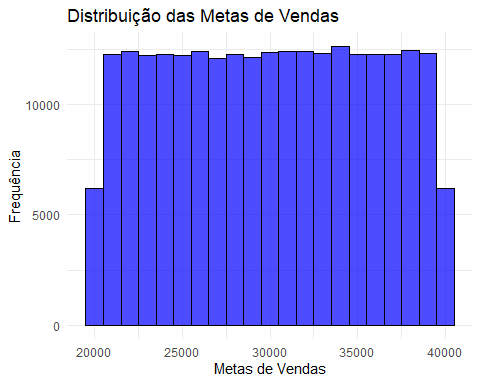
\includegraphics{Analize_exploratoria_files/figure-latex/unnamed-chunk-6-1.pdf}

\begin{Shaded}
\begin{Highlighting}[]
\FunctionTok{ggplot}\NormalTok{(targets\_salesperson\_final, }\FunctionTok{aes}\NormalTok{(}\AttributeTok{x =}\NormalTok{ .data[[sales\_target\_col]])) }\SpecialCharTok{+}
  \FunctionTok{geom\_density}\NormalTok{(}\AttributeTok{fill =} \StringTok{"blue"}\NormalTok{, }\AttributeTok{alpha =} \FloatTok{0.5}\NormalTok{) }\SpecialCharTok{+}
  \FunctionTok{theme\_minimal}\NormalTok{() }\SpecialCharTok{+}
  \FunctionTok{labs}\NormalTok{(}\AttributeTok{title =} \StringTok{"Densidade das Metas de Vendas"}\NormalTok{, }\AttributeTok{x =} \StringTok{"Metas de Vendas"}\NormalTok{, }\AttributeTok{y =} \StringTok{"Densidade"}\NormalTok{)}
\end{Highlighting}
\end{Shaded}

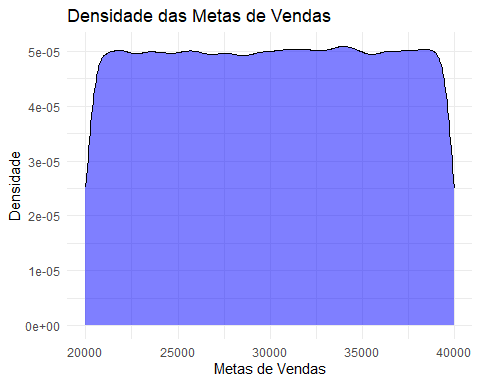
\includegraphics{Analize_exploratoria_files/figure-latex/unnamed-chunk-6-2.pdf}

\begin{Shaded}
\begin{Highlighting}[]
\FunctionTok{ggplot}\NormalTok{(targets\_salesperson\_final, }\FunctionTok{aes}\NormalTok{(}\AttributeTok{y =}\NormalTok{ .data[[sales\_target\_col]])) }\SpecialCharTok{+}
  \FunctionTok{geom\_boxplot}\NormalTok{(}\AttributeTok{fill =} \StringTok{"blue"}\NormalTok{, }\AttributeTok{alpha =} \FloatTok{0.7}\NormalTok{) }\SpecialCharTok{+}
  \FunctionTok{theme\_minimal}\NormalTok{() }\SpecialCharTok{+}
  \FunctionTok{labs}\NormalTok{(}\AttributeTok{title =} \StringTok{"Boxplot das Metas de Vendas"}\NormalTok{, }\AttributeTok{y =} \StringTok{"Metas de Vendas"}\NormalTok{)}
\end{Highlighting}
\end{Shaded}

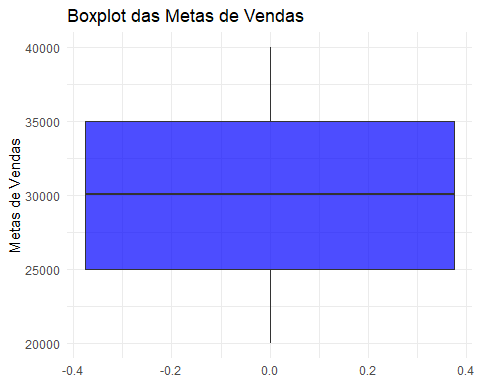
\includegraphics{Analize_exploratoria_files/figure-latex/unnamed-chunk-6-3.pdf}

\begin{Shaded}
\begin{Highlighting}[]
\NormalTok{identify\_outliers }\OtherTok{\textless{}{-}} \ControlFlowTok{function}\NormalTok{(data, variable, }\AttributeTok{factor =} \FloatTok{1.5}\NormalTok{) \{}
\NormalTok{  Q1 }\OtherTok{\textless{}{-}} \FunctionTok{quantile}\NormalTok{(data[[variable]], }\FloatTok{0.25}\NormalTok{, }\AttributeTok{na.rm =} \ConstantTok{TRUE}\NormalTok{)}
\NormalTok{  Q3 }\OtherTok{\textless{}{-}} \FunctionTok{quantile}\NormalTok{(data[[variable]], }\FloatTok{0.75}\NormalTok{, }\AttributeTok{na.rm =} \ConstantTok{TRUE}\NormalTok{)}
\NormalTok{  IQR }\OtherTok{\textless{}{-}}\NormalTok{ Q3 }\SpecialCharTok{{-}}\NormalTok{ Q1}
\NormalTok{  lower\_bound }\OtherTok{\textless{}{-}}\NormalTok{ Q1 }\SpecialCharTok{{-}}\NormalTok{ factor }\SpecialCharTok{*}\NormalTok{ IQR}
\NormalTok{  upper\_bound }\OtherTok{\textless{}{-}}\NormalTok{ Q3 }\SpecialCharTok{+}\NormalTok{ factor }\SpecialCharTok{*}\NormalTok{ IQR}
\NormalTok{  outliers }\OtherTok{\textless{}{-}}\NormalTok{ data }\SpecialCharTok{\%\textgreater{}\%} \FunctionTok{filter}\NormalTok{(data[[variable]] }\SpecialCharTok{\textless{}}\NormalTok{ lower\_bound }\SpecialCharTok{|}\NormalTok{ data[[variable]] }\SpecialCharTok{\textgreater{}}\NormalTok{ upper\_bound)}
  \FunctionTok{return}\NormalTok{(outliers)}
\NormalTok{\}}

\NormalTok{outliers\_sales\_target }\OtherTok{\textless{}{-}} \FunctionTok{identify\_outliers}\NormalTok{(targets\_salesperson\_final, }\StringTok{"sales\_target"}\NormalTok{, }\DecValTok{2}\NormalTok{)}

\FunctionTok{print}\NormalTok{(}\StringTok{"Outliers nas Metas de Vendas com fator 2:"}\NormalTok{)}
\end{Highlighting}
\end{Shaded}

\begin{verbatim}
## [1] "Outliers nas Metas de Vendas com fator 2:"
\end{verbatim}

\begin{Shaded}
\begin{Highlighting}[]
\FunctionTok{print}\NormalTok{(outliers\_sales\_target)}
\end{Highlighting}
\end{Shaded}

\begin{verbatim}
## [1] id_employee  sales_target month       
## <0 linhas> (ou row.names de comprimento 0)
\end{verbatim}

Outliers: Com o calculo do interquartil não foi encontrado nenhum
outliers.

1.3. - Análise Bivariada:

\begin{Shaded}
\begin{Highlighting}[]
\FunctionTok{ggplot}\NormalTok{(targets\_salesperson\_final, }\FunctionTok{aes}\NormalTok{(}\AttributeTok{x =}\NormalTok{ month, }\AttributeTok{y =}\NormalTok{ sales\_target, }\AttributeTok{color =} \FunctionTok{factor}\NormalTok{(id\_employee))) }\SpecialCharTok{+}
  \FunctionTok{geom\_point}\NormalTok{(}\AttributeTok{alpha =} \FloatTok{0.7}\NormalTok{) }\SpecialCharTok{+}
  \FunctionTok{theme\_minimal}\NormalTok{() }\SpecialCharTok{+}
  \FunctionTok{labs}\NormalTok{(}\AttributeTok{title =} \StringTok{"Relação entre Metas de Vendas e Mês"}\NormalTok{,}
       \AttributeTok{x =} \StringTok{"Mês"}\NormalTok{,}
       \AttributeTok{y =} \StringTok{"Metas de Vendas"}\NormalTok{,}
       \AttributeTok{color =} \StringTok{"ID do Funcionário"}\NormalTok{)}
\end{Highlighting}
\end{Shaded}

\includegraphics{Analize_exploratoria_files/figure-latex/unnamed-chunk-7-1.pdf}

\begin{Shaded}
\begin{Highlighting}[]
\FunctionTok{ggplot}\NormalTok{(targets\_salesperson\_final, }\FunctionTok{aes}\NormalTok{(}\AttributeTok{x =}\NormalTok{ month, }\AttributeTok{y =}\NormalTok{ sales\_target, }\AttributeTok{fill =} \FunctionTok{factor}\NormalTok{(id\_employee))) }\SpecialCharTok{+}
  \FunctionTok{geom\_bar}\NormalTok{(}\AttributeTok{stat =} \StringTok{"identity"}\NormalTok{, }\AttributeTok{position =} \StringTok{"dodge"}\NormalTok{) }\SpecialCharTok{+}
  \FunctionTok{theme\_minimal}\NormalTok{() }\SpecialCharTok{+}
  \FunctionTok{labs}\NormalTok{(}\AttributeTok{title =} \StringTok{"Distribuição das Metas de Vendas por Mês"}\NormalTok{,}
       \AttributeTok{x =} \StringTok{"Mês"}\NormalTok{,}
       \AttributeTok{y =} \StringTok{"Metas de Vendas"}\NormalTok{,}
       \AttributeTok{fill =} \StringTok{"ID do Funcionário"}\NormalTok{)}
\end{Highlighting}
\end{Shaded}

\includegraphics{Analize_exploratoria_files/figure-latex/unnamed-chunk-7-2.pdf}

\begin{Shaded}
\begin{Highlighting}[]
\NormalTok{correlation\_matrix }\OtherTok{\textless{}{-}} \FunctionTok{cor}\NormalTok{(targets\_salesperson\_final }\SpecialCharTok{\%\textgreater{}\%} \FunctionTok{select}\NormalTok{(sales\_target))}

\FunctionTok{library}\NormalTok{(corrplot)}


\NormalTok{numeric\_vars }\OtherTok{\textless{}{-}}\NormalTok{ targets\_salesperson\_final }\SpecialCharTok{\%\textgreater{}\%}
  \FunctionTok{select}\NormalTok{(}\FunctionTok{where}\NormalTok{(is.numeric))}

\NormalTok{correlation\_matrix }\OtherTok{\textless{}{-}} \FunctionTok{cor}\NormalTok{(numeric\_vars, }\AttributeTok{use =} \StringTok{"complete.obs"}\NormalTok{)}

\FunctionTok{corrplot}\NormalTok{(correlation\_matrix, }\AttributeTok{method =} \StringTok{"circle"}\NormalTok{, }\AttributeTok{type =} \StringTok{"upper"}\NormalTok{, }\AttributeTok{tl.cex =} \FloatTok{0.8}\NormalTok{, }\AttributeTok{title =} \StringTok{"Matriz de Correlação"}\NormalTok{)}
\end{Highlighting}
\end{Shaded}

\includegraphics{Analize_exploratoria_files/figure-latex/unnamed-chunk-7-3.pdf}

1.4. - Análise Multivariada:

\begin{Shaded}
\begin{Highlighting}[]
\NormalTok{numeric\_vars }\OtherTok{\textless{}{-}}\NormalTok{ targets\_salesperson\_final }\SpecialCharTok{\%\textgreater{}\%}
  \FunctionTok{select}\NormalTok{(}\FunctionTok{where}\NormalTok{(is.numeric))}

\NormalTok{scaled\_data }\OtherTok{\textless{}{-}} \FunctionTok{scale}\NormalTok{(numeric\_vars)}

\NormalTok{pca\_result }\OtherTok{\textless{}{-}} \FunctionTok{prcomp}\NormalTok{(scaled\_data, }\AttributeTok{center =} \ConstantTok{TRUE}\NormalTok{, }\AttributeTok{scale. =} \ConstantTok{TRUE}\NormalTok{)}

\FunctionTok{fviz\_pca\_biplot}\NormalTok{(pca\_result, }
                \AttributeTok{geom.ind =} \StringTok{"point"}\NormalTok{, }
                \AttributeTok{pointshape =} \DecValTok{21}\NormalTok{, }
                \AttributeTok{pointsize =} \FloatTok{2.5}\NormalTok{,}
                \AttributeTok{fill.ind =}\NormalTok{ targets\_salesperson\_final}\SpecialCharTok{$}\NormalTok{id\_employee, }
                \AttributeTok{col.ind =} \StringTok{"black"}\NormalTok{, }
                \AttributeTok{palette =} \StringTok{"jco"}\NormalTok{,}
                \AttributeTok{addEllipses =} \ConstantTok{TRUE}\NormalTok{,}
                \AttributeTok{label =} \StringTok{"var"}\NormalTok{,}
                \AttributeTok{col.var =} \StringTok{"blue"}\NormalTok{,}
                \AttributeTok{repel =} \ConstantTok{TRUE}\NormalTok{,}
                \AttributeTok{title =} \StringTok{"Biplot da Análise de Componentes Principais (PCA)"}
\NormalTok{)}
\end{Highlighting}
\end{Shaded}

\begin{verbatim}
## Warning: Computation failed in `stat_ellipse()`.
## Caused by error in `chol.default()`:
## ! the leading minor of order 2 is not positive
\end{verbatim}

\includegraphics{Analize_exploratoria_files/figure-latex/unnamed-chunk-8-1.pdf}

1.5. - Conclusão da análise:

\end{document}
